\section{Small signal pump measurements}
\label{sec:small_sig_pump}

In this section the linear small signal deviation of the linearized pump model is measured and calculated.


%\subsection{One clamp push} % \label{app:...}
\subsection*{Test equipment:}
\begin{itemize}
\item The water distribution system at AAU.
\end{itemize}

\subsection*{Procedure:}
The following procedure was made for finding the small signal deviations of the pumps
\begin{enumerate}
\item Wait for the system to reach the steady state operating point.
\item Add $\pm 0.05\omega$ to the rotational speed for one of the pumps and wait 30 minutes for steady state.
\item Note differential pressure over the pump, set the rotational speed to the operating point and 30 minutes to reach operating steady state. 
\end{enumerate}
Point 2-3 is done for each pump where the pressure over the pump is noted 

\subsection*{Measuring data:}
The data from the measurements can be seen on 

\todo{edit the rest - Simon}

% \begin{figure}[H]
% % This file was created by matlab2tikz.
%
%The latest updates can be retrieved from
%  http://www.mathworks.com/matlabcentral/fileexchange/22022-matlab2tikz-matlab2tikz
%where you can also make suggestions and rate matlab2tikz.
%
\definecolor{mycolor1}{rgb}{0.00000,0.44700,0.74100}%
%
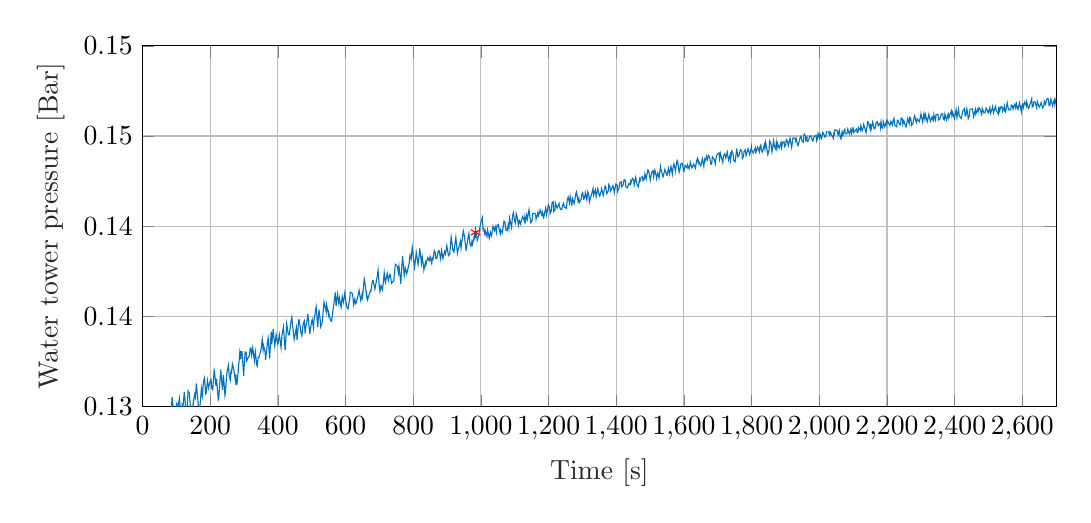
\begin{tikzpicture}

\begin{axis}[%
width=4.568in,
height=1.803in,
at={(0.766in,0.486in)},
scale only axis,
xmin=0,
xmax=2700,
xlabel style={font=\color{white!15!black}},
xlabel={Time [s]},
ymin=0.13,
ymax=0.15,
ylabel style={font=\color{white!15!black}},
ylabel={Water tower pressure [Bar] },
axis background/.style={fill=white},
xmajorgrids,
ymajorgrids
]
\addplot [color=mycolor1, forget plot]
  table[row sep=crcr]{%
0	0.127664975562129\\
0.1	0.12764670576741\\
6.25	0.128835982404655\\
6.25	0.128835982404655\\
10.25	0.1281182404692\\
14.1	0.128942121212128\\
18.75	0.127501417399822\\
18.75	0.127501417399822\\
23.85	0.128946471163334\\
25.05	0.128727233626671\\
29.8	0.128004271749825\\
31.25	0.1282922385142\\
35.1	0.129446715542429\\
38.45	0.129071749755616\\
43.4	0.128629794721434\\
46.85	0.129277067448709\\
50	0.128632404692115\\
50.1	0.128590645161313\\
55.1	0.129464985337262\\
58.9	0.128590645161256\\
62.5	0.129266627566028\\
63.95	0.129656383186773\\
68.75	0.128414037145615\\
68.9	0.128329648093813\\
73.9	0.129231827957034\\
75.45	0.128789872922783\\
81	0.129668563049881\\
82.95	0.129276197458466\\
87.45	0.130527243401792\\
87.5	0.130508103616847\\
92.2	0.129605923753695\\
96.05	0.129672913001002\\
99.2	0.13003395894425\\
101.05	0.130151407624663\\
102.4	0.129701622678448\\
108.85	0.130444594330413\\
112.5	0.129712932551359\\
114.15	0.129262277614919\\
116.85	0.13002525904206\\
118.75	0.129835601173068\\
123.45	0.13079955034209\\
125	0.130490703812274\\
129.8	0.129298817204312\\
131.25	0.12976948191594\\
134.65	0.130863059628575\\
138.2	0.130733431085025\\
143.1	0.129611143695018\\
146.3	0.129592003910039\\
149.7	0.130190557184756\\
150	0.130152277614872\\
153.55	0.130666441837809\\
156.25	0.130493313783035\\
159	0.131268475073301\\
162.5	0.130569002932509\\
166.3	0.129703362658876\\
168.8	0.129806891495633\\
173.9	0.13099007820137\\
176.7	0.130579442815338\\
180.5	0.131422463343159\\
183.25	0.131589501466323\\
186.6	0.130705591397901\\
188.3	0.130765620723395\\
191.8	0.131432033235603\\
195.1	0.131026617790826\\
199.3	0.131365043988319\\
202.4	0.131485102639357\\
204.75	0.130980508308869\\
207.4	0.130925698924716\\
211.75	0.132013186705757\\
212.5	0.131956637341165\\
216.95	0.131144066471177\\
218.75	0.131545131964839\\
223.7	0.13037412512225\\
225.15	0.130455904203336\\
231.15	0.132036676441879\\
231.25	0.132009706744907\\
236.1	0.130923958944243\\
239.05	0.13173217986307\\
243.55	0.130604672531791\\
244.05	0.13065426197461\\
249.7	0.131923577712638\\
253.85	0.132283753665689\\
256	0.131720000000001\\
259.2	0.1314616129032\\
261.75	0.132040156402735\\
262.65	0.131788729227748\\
265.5	0.132356832844619\\
268.9	0.13211410557189\\
274.6	0.131415503421363\\
275.8	0.131773939393918\\
278.65	0.131199745845458\\
281.25	0.131661710654942\\
287.4	0.132990185728295\\
290	0.132608260019538\\
290.95	0.133044995112425\\
294.05	0.133027595307897\\
298.95	0.131692160312775\\
300.05	0.132148905180838\\
303.25	0.133023245356753\\
306.25	0.133004975561948\\
307.85	0.132531700879701\\
315.75	0.13283271749757\\
317.85	0.13319115347017\\
319.85	0.133240742913029\\
322.5	0.132836197458425\\
325.6	0.13325901270764\\
330.5	0.132526480938395\\
333.3	0.133031075268798\\
337.3	0.132315073313748\\
339.05	0.132234164222757\\
341.45	0.132721358748722\\
343.75	0.13270830889544\\
350	0.133144173997982\\
353.65	0.133713147605079\\
356.25	0.133136344085995\\
357.8	0.133362541544409\\
362.5	0.132984965786943\\
363.55	0.132569980449671\\
368.7	0.133469550342079\\
371.15	0.133785356793794\\
375	0.132867517106536\\
375.5	0.132654369501415\\
380.25	0.134149882698011\\
381.8	0.133446930596313\\
386.25	0.134294301075124\\
387.45	0.133950654936359\\
390.9	0.133347751710676\\
394.75	0.133973274682296\\
399.15	0.133444320625563\\
400.45	0.133474770283385\\
404.2	0.133984584555196\\
409.35	0.133260752688216\\
411.95	0.133944565004902\\
416.4	0.134416099706709\\
418.7	0.13380536656897\\
421.45	0.133118074291326\\
424.95	0.134175112414505\\
426.05	0.134570957966685\\
431.1	0.13396544477024\\
434.05	0.13396892473105\\
437.05	0.134537898338112\\
441.25	0.134952013685302\\
443.7	0.134435239491779\\
443.7	0.134435239491779\\
448.25	0.133713147605033\\
454.5	0.134371730205191\\
456.2	0.133865395894372\\
456.65	0.133674868035143\\
461.5	0.134794545454531\\
462.95	0.134799765395894\\
468.3	0.134083763440947\\
470.8	0.133915855327496\\
474.95	0.134606627566006\\
478	0.134737126099753\\
480.5	0.134034173998032\\
481.2	0.134264721407578\\
487.45	0.134892854349937\\
488.35	0.135134711632497\\
493.65	0.134184682306807\\
493.95	0.134027214076127\\
499.95	0.134705806451564\\
501.4	0.134821515151464\\
505.25	0.134357810361792\\
506.3	0.134728426197591\\
512.4	0.135458347996087\\
513.05	0.135524467253208\\
517.7	0.134400439882768\\
518.75	0.134691016617808\\
521.4	0.135372218963812\\
524.95	0.134816295210226\\
526.4	0.134420449657864\\
531.2	0.134664046920818\\
536.2	0.135796774193568\\
537.75	0.135696725317757\\
542.75	0.135238240469232\\
543.9	0.135645395894414\\
549.7	0.135088602150472\\
550	0.135203440860153\\
556.15	0.134760615835671\\
558.7	0.134725816226671\\
562.45	0.135266080156441\\
562.45	0.135266080156441\\
568.7	0.136159560117233\\
569.35	0.136318768328408\\
572.1	0.135570576735131\\
576.2	0.136232639296236\\
580	0.135720215053755\\
582.05	0.136005571847545\\
586.8	0.135483577712557\\
587.45	0.135562746823018\\
590	0.136101270772201\\
593.8	0.135783724340183\\
597.85	0.13630832844575\\
599.95	0.135961202346095\\
603.4	0.135528817204283\\
607.3	0.135407018572846\\
612.45	0.13599252199416\\
612.45	0.13599252199416\\
614.15	0.136335298142785\\
620.5	0.136257869012695\\
623.9	0.135640175953063\\
627.4	0.135956852394872\\
630	0.135697595307897\\
631.3	0.135739354838756\\
637.45	0.136194359726403\\
640	0.136442306940444\\
643.2	0.136044721407575\\
644.95	0.135869853372355\\
648.75	0.136230899315751\\
650.2	0.136075171065488\\
655.1	0.137080879765404\\
656.65	0.136939071358688\\
662.2	0.136136070381144\\
662.7	0.136205669599144\\
665.05	0.135915092864116\\
668.7	0.136146510264007\\
673.65	0.136417947214045\\
674.95	0.136395327468233\\
679.55	0.136977350928737\\
681.55	0.136969521016783\\
686.7	0.13650146627574\\
688.65	0.136714613880736\\
693.7	0.137221818181774\\
696.15	0.137551544477003\\
699.85	0.136638054741002\\
701.7	0.136377057673633\\
704.75	0.13670330400787\\
709.25	0.136471016617759\\
712.45	0.137046080156381\\
714.2	0.137417565982412\\
718.15	0.136769423264968\\
718.7	0.13695647116333\\
723.1	0.137378416422246\\
726.35	0.136985180840668\\
730.6	0.137324477028267\\
732.6	0.137295767350975\\
735.65	0.136821622678383\\
742.95	0.136993880742875\\
743.7	0.137281847507313\\
743.75	0.137261837732149\\
747.1	0.137885620723455\\
753.2	0.137773391984388\\
756.2	0.137405386119178\\
758	0.137762952101639\\
762.4	0.136996490713523\\
763.1	0.13680509286404\\
768.4	0.138327575757546\\
769	0.138225786901216\\
773.4	0.13726009775171\\
776.45	0.137663773216093\\
780.65	0.137347966764492\\
781.3	0.13740016617802\\
787.4	0.137887360703769\\
787.4	0.137887360703769\\
790.5	0.138389345063524\\
793.85	0.138188377321637\\
797	0.138823470185628\\
800	0.13832844574772\\
803.85	0.137722062561181\\
806.35	0.138087458455516\\
808.85	0.138549423264897\\
814.35	0.137868220918915\\
818.65	0.138586832844589\\
819.35	0.13875909090907\\
824.35	0.137926510263992\\
826.55	0.13829625610955\\
831.15	0.137658553274559\\
831.45	0.137569814271637\\
835.95	0.137983059628505\\
837.4	0.137852561094826\\
842.65	0.138241446725226\\
847.15	0.138077888562941\\
849.65	0.13830843597259\\
854.7	0.137935210166211\\
856.1	0.138217086999066\\
858.35	0.138156187683273\\
862	0.138640772238409\\
864.7	0.138551163245324\\
866.85	0.138205777126063\\
869.35	0.138194467253072\\
874.05	0.138622502443809\\
876.3	0.138647732160314\\
881.05	0.138169237536692\\
881.15	0.138194467253209\\
883.7	0.138656432062589\\
887.7	0.138211867057646\\
892.65	0.13858857282496\\
895.3	0.138451114369411\\
899.25	0.138919169110579\\
900.2	0.138788670576798\\
904.25	0.138364985337103\\
907.9	0.138448504398878\\
912.05	0.13940375366567\\
912.4	0.13936286412511\\
917.05	0.138663391984426\\
920.3	0.138556383186744\\
924.9	0.139242805474021\\
925.85	0.139376783968714\\
930.5	0.138511143695075\\
931.15	0.138582482893435\\
936.3	0.138926129032393\\
939.65	0.139167116324757\\
941.35	0.138782580645284\\
943.65	0.139128836754651\\
948.05	0.139724780058452\\
951.25	0.139452473118092\\
956.05	0.13865730205282\\
956.15	0.13865730205282\\
962.4	0.13940636363626\\
964.7	0.139593411534577\\
967.6	0.139001818181839\\
970.6	0.138891329423245\\
973.4	0.139150586510277\\
975.25	0.138993118279518\\
981.15	0.13951598240476\\
982.25	0.139357644183849\\
984.5	0.139701290322671\\
987.4	0.139482052785797\\
989.25	0.139211485825899\\
993.65	0.139480312805438\\
997.6	0.140012746823072\\
1004.05	0.140473841642211\\
1006.1	0.13990225806449\\
1006.4	0.139924877810336\\
1011.5	0.139552521994256\\
1012.4	0.139770889540625\\
1017.95	0.139429853372405\\
1019.75	0.139780459433064\\
1024.85	0.139320234604054\\
1024.9	0.139323714564955\\
1028.05	0.139661270772228\\
1031.35	0.139464652981383\\
1035.6	0.139984907135852\\
1040.1	0.13974652981442\\
1042.5	0.139959677419404\\
1045.9	0.139658660801626\\
1047.15	0.140038846529785\\
1051.15	0.140082346041129\\
1056.05	0.139630821114372\\
1057.2	0.139574271749734\\
1058.3	0.139790029325502\\
1063.3	0.139631691104637\\
1068.25	0.140278963831906\\
1070.8	0.140225024437939\\
1074.1	0.139775239491712\\
1077.3	0.139738699902296\\
1080.5	0.140085826002019\\
1082.8	0.139854408602173\\
1084.75	0.1404425219941\\
1090.75	0.139911827956951\\
1093.2	0.140548660801562\\
1095.95	0.140740058651079\\
1099.35	0.140296363636332\\
1102.05	0.140166735092805\\
1104.35	0.140691339198406\\
1106.8	0.140543440860188\\
1110.85	0.140047546432015\\
1113.25	0.140305933528828\\
1116.95	0.140115405669621\\
1118.75	0.140268523949169\\
1123.7	0.140531260997079\\
1128.6	0.140274613880649\\
1129.95	0.140511251221835\\
1132	0.14026591397843\\
1135.2	0.140618260019437\\
1137.4	0.140392932551265\\
1142.05	0.140906226783989\\
1143.65	0.140665239491761\\
1147.45	0.140178914956084\\
1151.4	0.140302453567995\\
1152.85	0.140700909090981\\
1159.35	0.140713958944286\\
1162.35	0.140538220918791\\
1162.95	0.140381622678342\\
1168.5	0.140761808406694\\
1169.8	0.140564320625617\\
1174.55	0.140820097751623\\
1175.1	0.140885347018434\\
1180.25	0.140600860215079\\
1181.8	0.14077746823076\\
1185.6	0.140485151515145\\
1187.35	0.140633919843538\\
1191.3	0.141010625610966\\
1194.15	0.140626959921815\\
1199.2	0.141187233626511\\
1202.5	0.141054125122093\\
1204.5	0.140689599217956\\
1207.7	0.140823577712683\\
1210.2	0.141296852394839\\
1213.6	0.141353401759432\\
1215.2	0.14081922776146\\
1219.05	0.140921886608078\\
1220	0.141283802541568\\
1224.95	0.14100714564994\\
1231	0.141241173020649\\
1231.1	0.14121246334322\\
1234.8	0.140932326490713\\
1238.75	0.140919276637305\\
1243.55	0.141269882697941\\
1243.9	0.141276842619777\\
1246.45	0.141058475073294\\
1252.65	0.140983655914079\\
1255.2	0.14145171065494\\
1257.85	0.141612658846418\\
1261.7	0.141278582600125\\
1263.75	0.141654418377334\\
1268.6	0.141177663734106\\
1268.75	0.141121984359722\\
1270.6	0.141526529814246\\
1275.5	0.141247262952152\\
1281.1	0.141850166177778\\
1282.15	0.141904975562034\\
1286.9	0.141390811339147\\
1289.5	0.141544799608869\\
1290.6	0.141299462365464\\
1296.1	0.141479550342081\\
1298.35	0.14179796676442\\
1300.85	0.141867565982295\\
1303.55	0.14150478005854\\
1306.15	0.141542189638244\\
1308.6	0.141859736070364\\
1313.1	0.141462150537586\\
1316	0.141913675464275\\
1319.05	0.141745767350926\\
1320.55	0.141331652003851\\
1324.9	0.141627448680231\\
1331.1	0.142058093841729\\
1331.4	0.142083323558256\\
1333	0.14171966764419\\
1338.05	0.142018944281403\\
1340.5	0.141630928641246\\
1345.45	0.142078973606988\\
1349.85	0.141692697946996\\
1350.9	0.141663988269568\\
1355.8	0.141954565004812\\
1356.6	0.142072883675417\\
1361.65	0.141717927663717\\
1362.35	0.141802316715552\\
1367.05	0.142233831866884\\
1368.6	0.142186852394707\\
1372.15	0.141797966764466\\
1376.35	0.14196152492666\\
1377.6	0.142305171065323\\
1381.4	0.14217728250236\\
1382.55	0.141931945259046\\
1390.2	0.142241661778939\\
1393.4	0.141965874877701\\
1394.1	0.141851906158195\\
1398.8	0.142329530791801\\
1402.9	0.142272981427072\\
1403.85	0.141924115346944\\
1407.85	0.142104203323527\\
1410.65	0.142423489735882\\
1414.9	0.142460029325434\\
1415.65	0.142176412512163\\
1419.9	0.142269501466205\\
1423.25	0.142577478005853\\
1426.85	0.1425296285434\\
1428.5	0.142169452590417\\
1432.4	0.142126823069475\\
1437.35	0.142353890518029\\
1440.3	0.142303431085111\\
1442.8	0.142490478983439\\
1443.6	0.14240173998046\\
1448	0.142647947214039\\
1451.2	0.14257747800591\\
1452.95	0.14227559139789\\
1457.55	0.142710586510213\\
1461.45	0.142290381231624\\
1465.1	0.142180762463192\\
1468.6	0.142599227761445\\
1470.05	0.142486999022435\\
1473.45	0.142683616813201\\
1478	0.142754956011618\\
1478.65	0.142512228738906\\
1482.95	0.142617497556114\\
1484.75	0.142903724340033\\
1488.2	0.142605317692926\\
1493.45	0.143120351906089\\
1495.6	0.143093382209111\\
1499.85	0.142643597262963\\
1500.5	0.142538328445812\\
1505.5	0.143036832844541\\
1509.5	0.143062932551288\\
1510.5	0.14274103616807\\
1514.15	0.143109912023363\\
1518.6	0.142746256109524\\
1519.1	0.142640987292316\\
1523	0.14295157380252\\
1526.45	0.142673176930577\\
1530.7	0.143286520039146\\
1531.1	0.143219530791805\\
1537.35	0.142777575757486\\
1538.6	0.142742776148486\\
1543.6	0.143143841642188\\
1543.6	0.143143841642188\\
1549	0.142834995112366\\
1550.1	0.142823685239352\\
1554.15	0.143203870967727\\
1557.3	0.142885454545535\\
1561.75	0.143311749755549\\
1565.6	0.142875884652915\\
1568.55	0.143310879765431\\
1570.3	0.14345529814276\\
1574.8	0.14309686217008\\
1574.85	0.143080332355817\\
1579.85	0.143656265884522\\
1581.1	0.1436414760508\\
1585.9	0.142991593352872\\
1587.5	0.143094252199376\\
1590.8	0.143448338220753\\
1594.75	0.143483137829708\\
1599.8	0.143022913000993\\
1599.85	0.143020303030323\\
1603.35	0.143365689149653\\
1609.25	0.143236930596277\\
1610.3	0.143411798631519\\
1615.3	0.143184731182714\\
1618.5	0.143483137829867\\
1618.85	0.14354577712603\\
1623.5	0.143223010752638\\
1624.8	0.143251720430112\\
1628.95	0.143443988269723\\
1634	0.143216920821101\\
1637.05	0.143608416422319\\
1639.9	0.143750224829034\\
1642.05	0.143497057673494\\
1643.55	0.143617116324549\\
1649.3	0.143340459432841\\
1650.3	0.143355249266676\\
1654.35	0.143738914955941\\
1658.8	0.143313489736033\\
1660.9	0.143678015640205\\
1662.3	0.143604936461281\\
1667.05	0.14388159335283\\
1668.65	0.143662355816195\\
1672.75	0.143916392961808\\
1676.3	0.14380242424229\\
1679.45	0.143427458455415\\
1681.8	0.143436158357599\\
1684.1	0.143838963831718\\
1689.3	0.143704985337115\\
1692.75	0.143464868035062\\
1693.6	0.14364321603116\\
1697.6	0.143955542521906\\
1703.95	0.144059071358731\\
1705.25	0.143739784946229\\
1707.9	0.144028621700863\\
1711.95	0.143714555229769\\
1714.75	0.143521417399779\\
1716.9	0.14390856304982\\
1720.8	0.144019051808516\\
1723.9	0.143771974584513\\
1728.1	0.144107790811211\\
1730.9	0.143766754643127\\
1731.95	0.143657135874787\\
1736.75	0.143952062560913\\
1737.85	0.143679755620587\\
1741.35	0.144165210166159\\
1745.3	0.144019921798565\\
1746.7	0.143658875855272\\
1751.05	0.143564046920665\\
1756.05	0.144265259042038\\
1756.1	0.144266129032269\\
1759.55	0.143835483870919\\
1762.3	0.143912043010664\\
1767.35	0.14423828934506\\
1771.1	0.144163470185617\\
1772.5	0.143744134897167\\
1776.3	0.143875503421259\\
1777.5	0.144131280547424\\
1781.4	0.144238289345105\\
1783.65	0.143910303030327\\
1789.5	0.144287008797562\\
1792.7	0.144094740957928\\
1794.5	0.143959022482886\\
1799.45	0.144388797653937\\
1799.8	0.144250469208168\\
1804.35	0.144053851417357\\
1811	0.144335728250155\\
1812.2	0.144022531769167\\
1812.3	0.144040801563881\\
1817.4	0.144384447702771\\
1823.3	0.144105180840597\\
1824.3	0.144387057673475\\
1827.25	0.144499286412542\\
1829	0.144200879765401\\
1832.25	0.144105180840734\\
1837.3	0.144507116324473\\
1839.35	0.144287878787816\\
1841	0.144647184750693\\
1843.55	0.144433167155444\\
1848.05	0.143960762463348\\
1851.7	0.144231329423235\\
1853.05	0.144722003910022\\
1856.75	0.144615865102628\\
1860.1	0.144121710654906\\
1865.05	0.144728963831892\\
1867.35	0.144409677419458\\
1870.85	0.144282658846578\\
1872.9	0.144648924731098\\
1874.8	0.144333118279565\\
1876.2	0.14461151515153\\
1881.35	0.144324418377221\\
1887	0.144651534701836\\
1888.45	0.144349648093782\\
1891.75	0.144641094819121\\
1895.8	0.144692424242396\\
1897.55	0.144410547409609\\
1900.8	0.144507986314898\\
1902.65	0.144802043010873\\
1906.05	0.144691554252199\\
1908.45	0.144462746823046\\
1913.45	0.144874252199406\\
1918.35	0.144368787878841\\
1918.55	0.144396627566027\\
1922.35	0.144896871945286\\
1929.7	0.144839452590429\\
1930.35	0.144642834799583\\
1931.6	0.144854242424231\\
1936.55	0.144465356793671\\
1937.6	0.144470576734955\\
1943.5	0.144920361681216\\
1946.05	0.144983870967701\\
1949.75	0.144691554252177\\
1953.05	0.144660234604066\\
1955	0.145104799608941\\
1959.45	0.145011710654944\\
1960.1	0.144768113392024\\
1963.7	0.144918621700845\\
1964.5	0.144700254154441\\
1968.5	0.144739403714641\\
1971.35	0.144982130987296\\
1975.15	0.145007360703778\\
1980.15	0.144721133919859\\
1981.7	0.144755063538605\\
1984.8	0.144968211143623\\
1990.6	0.145039550342108\\
1991.8	0.144711564027352\\
1994.05	0.14482118279567\\
1996.3	0.145139599217941\\
2000.95	0.144875122189626\\
2002.2	0.145110019550316\\
2006.9	0.144864682306888\\
2010.15	0.145197018572867\\
2013	0.145115239491656\\
2016.8	0.14492993157379\\
2018.9	0.144968211143714\\
2021.3	0.145230078201348\\
2027.4	0.145225728250296\\
2031	0.145030850439844\\
2031.05	0.145011710654899\\
2032.05	0.145220508308819\\
2041.5	0.14486381231676\\
2043.3	0.145224858259985\\
2043.95	0.145018670576655\\
2046	0.14534578690118\\
2052.8	0.145312727272631\\
2055.45	0.145045640273679\\
2059	0.145305767350953\\
2062.25	0.144916881720269\\
2064.1	0.144835972629357\\
2067.35	0.145231818181776\\
2069.95	0.145043900293149\\
2074.2	0.145355356793664\\
2075.65	0.145384066471058\\
2076.5	0.14512219941339\\
2081.7	0.145123939394011\\
2084.15	0.145377976539589\\
2088.8	0.145118719452569\\
2093.5	0.145384066471172\\
2094.95	0.145141339198392\\
2099.5	0.145438875855189\\
2099.8	0.145447575757407\\
2101.8	0.145184838709599\\
2110.35	0.145391896383103\\
2111.6	0.145204848484741\\
2114	0.145190928641273\\
2116.45	0.145468455522814\\
2121.5	0.145315337243051\\
2122.85	0.145570244378928\\
2126.75	0.145291847507178\\
2131	0.145551104593892\\
2131.4	0.145632013684735\\
2136.35	0.145319687194183\\
2138.25	0.145181358748437\\
2143.1	0.145789481915858\\
2144.5	0.145765992179622\\
2149.65	0.145438875854984\\
2151.05	0.145679863147348\\
2152.75	0.145328387096538\\
2157.7	0.145775562072254\\
2161.75	0.145417996089554\\
2164.6	0.145396246333894\\
2168.1	0.145727712610005\\
2171.45	0.145797311827914\\
2174.05	0.145564154447561\\
2179.85	0.145716402736912\\
2180.95	0.14549368523933\\
2182.5	0.145749462365507\\
2183.95	0.145479765395703\\
2187.6	0.145428435972599\\
2188.95	0.14580340175944\\
2193.65	0.145509345063306\\
2198.2	0.145799921798516\\
2199.8	0.145647673509302\\
2200.95	0.145852991202355\\
2208.7	0.145577204300935\\
2211.55	0.14580688172025\\
2215.95	0.14560939393923\\
2218.25	0.145873870967534\\
2220.95	0.145975659823944\\
2222.75	0.145602434017724\\
2228.8	0.145509345063442\\
2230.55	0.145864301075176\\
2232.2	0.145882570869958\\
2236.75	0.14564419354856\\
2239.85	0.145616353861101\\
2241.85	0.145995669599188\\
2245.55	0.145936510263709\\
2246.95	0.145643323557829\\
2250	0.145841681329171\\
2254.95	0.145548494623449\\
2256.4	0.145504125121965\\
2261.6	0.14597913978464\\
2265.7	0.145689433039774\\
2267.55	0.146035689149221\\
2270.45	0.145972179863065\\
2272.6	0.145591994134884\\
2277.05	0.145707702834693\\
2280.25	0.146029599218082\\
2281.95	0.146125298142692\\
2287.05	0.145713792766355\\
2287.5	0.145714662756654\\
2289.4	0.145947820136894\\
2295.7	0.145797311827732\\
2299.75	0.146105288367335\\
2300.45	0.146220127077027\\
2305.5	0.145770342130868\\
2309.4	0.146236656891233\\
2312	0.145946950146231\\
2313.85	0.146188807428871\\
2318.15	0.14583820136836\\
2318.85	0.145781652003666\\
2323.85	0.146200117302033\\
2324.7	0.146085278592341\\
2328.5	0.145811231671405\\
2333.35	0.146061788856377\\
2336.7	0.14583124144674\\
2337.8	0.145876480938364\\
2338.65	0.14618445747783\\
2343.65	0.145870391006724\\
2344.65	0.146167057673529\\
2350.75	0.146199247311597\\
2352.55	0.145885180840583\\
2356.1	0.145924330400703\\
2361.1	0.146243616813058\\
2364.85	0.146208817204047\\
2366.6	0.145940860214932\\
2369.4	0.145894750733009\\
2371.2	0.146216647116171\\
2376.2	0.145879960899106\\
2380.95	0.146230566959639\\
2381.15	0.146294076246022\\
2382.65	0.145998279569744\\
2390.5	0.146392385141667\\
2392	0.146110508308766\\
2394.35	0.146301906158146\\
2399.3	0.145959130009578\\
2400.25	0.146038299120119\\
2404.35	0.146465464320568\\
2406.9	0.146029599217854\\
2411.6	0.146489824046739\\
2412.25	0.146390645161137\\
2413.6	0.146133998044911\\
2419.45	0.145969569892463\\
2424.4	0.146390645160932\\
2429.2	0.146523753665565\\
2430.95	0.146121818181632\\
2432.8	0.146110508308766\\
2436.1	0.146508093841476\\
2438	0.146322785923553\\
2440.15	0.145959999999855\\
2443.85	0.146135738025168\\
2445.15	0.146481124144452\\
2452.25	0.146500263929443\\
2455.95	0.146122688172022\\
2456.1	0.146084408602087\\
2461.1	0.146466334310776\\
2462.6	0.146213167155361\\
2467.2	0.146484604105558\\
2469.25	0.146347145650066\\
2472.15	0.146570733137628\\
2475.2	0.146487214075978\\
2480.2	0.146194027370461\\
2481.65	0.146533323558037\\
2486.6	0.146279286412369\\
2489.8	0.146305386119229\\
2493.1	0.146546373411411\\
2494.3	0.14649765395875\\
2499.3	0.146286246333966\\
2503.9	0.146579433039915\\
2505.55	0.146235786901229\\
2507.6	0.146322785923735\\
2512.15	0.146624672531675\\
2512.2	0.146607272727192\\
2515.1	0.146287116324288\\
2520.65	0.146632502443572\\
2523.35	0.146402825024234\\
2529.35	0.146213167155224\\
2530.75	0.146636852394818\\
2532.05	0.146354105571663\\
2537	0.146627282502209\\
2539.7	0.146623802541376\\
2542	0.146366285434829\\
2547.05	0.146656862169903\\
2548	0.146377595307695\\
2550.4	0.146322785923576\\
2555.4	0.14682825024438\\
2556	0.146749081134067\\
2559.35	0.146457634408671\\
2565.25	0.146444584555229\\
2567.65	0.14671689149543\\
2570.65	0.146685571847388\\
2572.75	0.146483734115213\\
2577.75	0.146763870967493\\
2580.55	0.146547243401346\\
2582.6	0.146783010752279\\
2586.85	0.146476774193457\\
2587.25	0.146465464320522\\
2591.8	0.14683956011711\\
2597.1	0.146341925708475\\
2598.75	0.146694271749584\\
2601.55	0.146760391006728\\
2602.85	0.146565513196379\\
2607.25	0.146882189638086\\
2612.2	0.146648162267888\\
2612.95	0.146884799609097\\
2618.3	0.146515923753554\\
2618.6	0.146517663734016\\
2624.25	0.146847390029257\\
2627.85	0.147071847507232\\
2629.25	0.14660553274673\\
2632.85	0.146669912023367\\
2633.7	0.146886539589309\\
2637.6	0.146888279569703\\
2642.55	0.146559423265012\\
2644.25	0.146914379276814\\
2649.2	0.146643812316597\\
2650.85	0.146599442815273\\
2655.85	0.146852609970551\\
2656.2	0.14683695014653\\
2659.85	0.14655594330402\\
2663.8	0.14666904203325\\
2664.95	0.146935259042016\\
2668.45	0.146768220918761\\
2673.15	0.147074457478016\\
2677.05	0.147053577712654\\
2679.15	0.146679481915885\\
2681.75	0.146711671554135\\
2684.45	0.14703704789838\\
2689.7	0.146674261974499\\
2693.2	0.146944828934534\\
2694.7	0.147018778103597\\
2696.25	0.146747341153332\\
2701	0.147169286412372\\
2705.95	0.146916989247097\\
2712.15	0.146781270772181\\
};
\addplot [color=red, draw=none, mark=asterisk, mark options={solid, red}, forget plot]
  table[row sep=crcr]{%
984.3	0.139652570870066\\
};
\end{axis}
\end{tikzpicture}%
% \caption{The data measurement for the finding the time constant of the WT. A small red dot shows the time constant for the tank which is 1155 seconds.}
% \label{fig:Test_WT_Timeconstant}
% \end{figure}

\subsection*{Results:}
The steady state differential pressure for time $[1800, 3600, 7200, 9000, 10800 12600, 16200, 18000]$ is noted and used for the small signal deviation. These values has been picked as this is the time when the signal to one of the pumps are change and where the differential pressure over the pump should have reached a reasonable steady state. The differential pressure shown in \eqref{eq:smallsig_differential_pressure}, is show with respect to $\omega + \hat{\omega}$ and $\omega + \bar{\omega}$

\begin{equation}
	\begin{split}
	\Delta P_{C_2} &= \wedge \\
	\Delta P_{C_{16}} &= \wedge \\
	\Delta P_{C_{18}} &= \wedge \\
	\Delta P_{C_{25}} &= \wedge
	\end{split}
	\label{eq:smallsig_differential_pressure}
\end{equation}

From these results, the small signal pressure can be derived as see in \eqref{eq:smallsig_diff_pres1} to \eqref{eq:smallsig_diff_pres4}.

\begin{equation}
\frac{\hat{\Delta P_{C_2}}}{\hat{\omega_{C_2}}} = \frac{Nan-Nan}{0.45-0.35} = Nan 
\label{eq:smallsig_diff_pres1}
\end{equation}

\begin{equation}
\frac{\hat{\Delta P_{C_16}}}{\hat{\omega_{C_2}}} = \frac{Nan-Nan}{0.45-0.35} = Nan 
\label{eq:smallsig_diff_pres2}
\end{equation}

\begin{equation}
\frac{\hat{\Delta P_{C_18}}}{\hat{\omega_{C_2}}} = \frac{Nan-Nan}{1.21 - 0.16} = Nan 
\label{eq:smallsig_diff_pres3}
\end{equation}

\begin{equation}
\frac{\hat{\Delta P_{C_25}}}{\hat{\omega_{C_2}}} = \frac{Nan-Nan}{0.45-0.35} = Nan 
\label{eq:smallsig_diff_pres4}
\end{equation}


\subsection*{Uncertainties of measurement:}
\begin{itemize}
\item The settling time for the initial state was not reached after 0.5 hours.
\item Corrupt pressure measurements or noise. 
\end{itemize}

\subsection*{Conclusion:}
From these measurements the small signal deviations have been found and will be used in the linearized small signal model for the pumps. 


